\section{Motivation}\label{subsec:motivation}

\begin{figure}[t]
  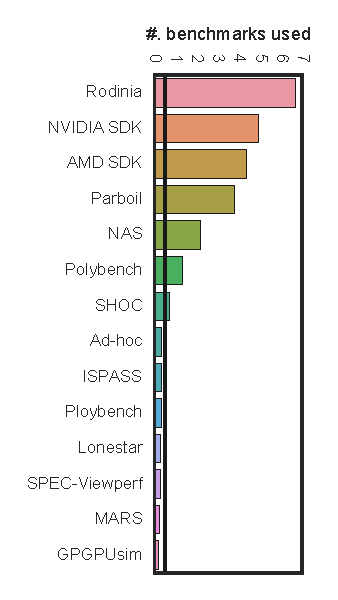
\includegraphics[width=\columnwidth]{img/motivation-c} %
  \caption{%
    The average number of benchmarks used in GPGPU research papers, organized by
    origin. In this work we use the seven most popular benchmark suites.%
  }%
  \label{fig:benchmark-suite-distribution}
\end{figure}

\begin{table*}
  \scriptsize%
  \centering%
  \begin{tabular}{ R{1.5cm} C{1.5cm} C{1.5cm} C{1.5cm} C{1.5cm} C{1.5cm} C{1.5cm} C{1.5cm} }
    \toprule
    & \textbf{AMD} & \textbf{NPB} & \textbf{NVIDIA} & \textbf{Parboil} & \textbf{Polybench} & \textbf{Rodinia} & \textbf{SHOC}\\
    \midrule
    \textbf{AMD} & - & 38.0\% & 74.5\% & 76.7\% & 21.7\% & 45.8\% & 35.9\%\\
    \textbf{NPB} & 22.7\% & - & 45.3\% & 36.7\% & 13.4\% & 16.1\% & 23.7\%\\
    \textbf{NVIDIA} & 29.9\% & 37.9\% & - & 21.8\% & 78.3\% & 18.1\% & 63.2\%\\
    \textbf{Parboil} & 89.2\% & 28.2\% & 28.2\% & - & 41.3\% & 73.0\% & 33.8\%\\
    \textbf{Polybench} & 58.6\% & 30.8\% & 45.3\% & 11.5\% & - & 43.9\% & 12.1\%\\
  \textbf{Rodinia} & 39.8\% & 36.4\% & 29.7\% & 36.5\% & 46.1\% & - & 59.9\%\\
  \textbf{SHOC} & 42.9\% & 71.5\% & 74.1\% & 41.4\% & 35.7\% & 81.0\% & -\\
  \end{tabular}
  \caption{Performance relative to the optimal of the \emph{Grewe et al.\ }predictive model across different benchmark suites on an AMD GPU. The columns show the suite used for training; the rows show the suite used for testing.}%
  \label{tab:benchmark-xval}
\end{table*}

In this section we make the argument for synthetic benchmarks. We identified frequently used benchmark suites in a survey of 25 research papers in the field of GPGPU performance tuning from four top tier conferences between 2013--2016: CGO, HiPC, PACT, and PPoPP. We found the average number of benchmarks used in each paper to be 17, and that a small pool of benchmarks suites account for the majority of results, shown in Figure~\ref{fig:benchmark-suite-distribution}. We selected the 7 most frequently used benchmark suites (accounting for 92\% of results), and evaluated the performance of the state of the art \emph{Grewe et   al.}~\cite{Grewe2013} predictive model across each. The model predicts whether running a given OpenCL kernel on the GPU gives better performance than on the CPU. We describe the full experimental methodology in Section~\ref{sec:methodology}.

Table~\ref{tab:benchmark-xval} summarizes our results. The performance of a model trained on one benchmark suite and used to predict the mapping for another suite is generally very poor. The benchmark suite which provides the best results, NVIDIA SDK, achieves on average only 49\% of the optimal performance. The worst case is when training with Parboil to predict the optimal mappings for Polybench, where the model achieves only 11.5\% of the optimal performance. From this it is clear that heuristics learned on one benchmark suite fail to generalize across other suites.

This problem is caused both by the limited number of benchmarks contained in each suite, and the distribution of benchmarks within the feature space. Figure~\ref{fig:pca-benchmarks} shows the feature space of the Parboil benchmark suite, showing whether, for each benchmark, the model was able to correctly predict the appropriate optimization.  We used Principle Component Analysis to reduce the multi-dimensional feature space to aid visualization.

As we see in Figure~\ref{fig:pca-benchmarks-a}, there is a dense cluster of neighboring benchmarks, a smaller cluster of three benchmarks, and two outliers. The lack of neighboring observations means that the model is unable to learn a good heuristic for the two outliers, which leads to them being incorrectly optimized. In Figure~\ref{fig:pca-benchmarks-b}, we hand-selected benchmarks which are neighbouring in the feature space and retrained the model. The addition of these observations (and the information they provide about that part of the feature space) causes the two outliers to be correctly optimized. We found such outliers in all of the benchmark suites of Table~\ref{tab:benchmark-xval}.

\begin{figure}
  \subfloat[]{%
    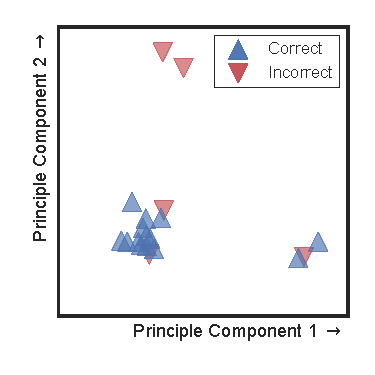
\includegraphics[width=.45\columnwidth]{img/motivation-a}%
    \label{fig:pca-benchmarks-a}%
  }%
  \subfloat[]{%
    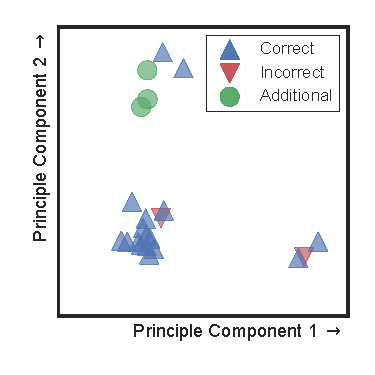
\includegraphics[width=.45\columnwidth]{img/motivation-b}%
    \label{fig:pca-benchmarks-b}%
  }%
  \caption{A two dimensional projection of the \emph{Grewe et al.\ } feature space, showing predictive model results over Parboil benchmarks on an NVIDIA GPU. Two outliers in~\protect\subref{fig:pca-benchmarks-a} are incorrectly predicted due to the lack of nearby observations. The addition of neighboring observations in~\protect\subref{fig:pca-benchmarks-b} corrects this.}%
  \label{fig:pca-benchmarks}
\end{figure}

These results highlight the significant effect that the number and distribution of training programs has on the quality of predictive models. Without good coverage of the feature space, any machine learning methodology is unlikely to produce high quality heuristics, suitable for general use on arbitrary real applications, or even applications from different benchmark suites. Our novel approach, described in the next section, solves this problem by generating an unbounded number of programs to cover the feature space with fine granularity.